\documentclass[12pt,letterpaper]{article}

% Typography
\usepackage{fontspec}
\usepackage{ebgaramond}

% Section and Subsection Formatting
\usepackage{titlesec}
\titleformat{\section}
  {\normalfont\fontsize{18}{15}\selectfont\bfseries}
  {\thesection}{6 pt}{}
\titleformat{\subsection}
  {\normalfont\fontsize{14}{13}\itshape\mdseries}
  {\thesubsection}{8 pt}{}

% Fonts
\newfontfamily\englishtowne{EnglishTowne}[
  Path = fonts/,
  Extension = .ttf,
]
\newfontfamily\anglican{AnglicanText-Regular}[
    Path = fonts/,
    Extension = .ttf,
]

% Page Layout
\usepackage{geometry}
\geometry{margin= 2cm} % Adjust as needed

% Graphics
\usepackage{graphicx}

% Text Formatting
\usepackage{parskip}
\usepackage{lipsum} % For generating dummy text
\usepackage[english]{babel}
\usepackage{soul}

% Colors
\usepackage{xcolor}
\definecolor{codegreen}{rgb}{0,0.6,0}
\definecolor{codegray}{rgb}{0.5,0.5,0.5}
\definecolor{codepurple}{rgb}{0.58,0,0.82}
\definecolor{backcolour}{rgb}{0.95,0.95,0.92}
\definecolor{tudelftdarkblue}{RGB}{12,35,64}
\definecolor{tudelftcyan}{RGB}{0,166,214}
\definecolor{tudelftblue}{RGB}{0,118,194}
\definecolor{tyrianpurple}{RGB}{95, 34, 68}
\definecolor{carlet}{RGB}{104, 22, 45}
\definecolor{indigoDye}{RGB}{8, 71, 120}
\definecolor{Denim}{RGB}{8, 93, 191}
\definecolor{faded-blue}{RGB}{78, 119, 166}
\definecolor{bluish-denim}{RGB}{5, 147, 255}
% Hyperlinks
\usepackage{hyperref}
\hypersetup{
    colorlinks=true, % Use color for links
    linkcolor=faded-blue, % Set link color
    urlcolor=Denim, % Set URL color
    citecolor=bluish-denim, % Set citation color
}

% Headers and Footers
\usepackage{fancyhdr}
\pagestyle{fancy}
\fancyhf{} % Clear header and footer
\renewcommand{\headrulewidth}{0pt} % Remove header line
\renewcommand{\footrulewidth}{0.5pt} % Add footer line
\fancyfoot[C]{\thepage} % Page number in the center of the footer

% Code Listings
\usepackage{listings}
\lstdefinestyle{mystyle}{
    backgroundcolor=\color{backcolour},   
    commentstyle=\color{codegreen},
    keywordstyle=\color{magenta},
    numberstyle=\tiny\color{codegray},
    stringstyle=\color{codepurple},
    basicstyle=\ttfamily\small,
    breakatwhitespace=false,         
    breaklines=true,                 
    captionpos=b,                    
    keepspaces=true,                 
    numbers=left,                    
    numbersep=5pt,                  
    showspaces=false,                
    showstringspaces=false,
    showtabs=false,                  
    tabsize=2
}
\lstset{style=mystyle}

% Algorithms
\usepackage{algpseudocode}

% Mathematics
\usepackage{amsmath}

% Loops
\usepackage{forloop}

% Tables
\usepackage{booktabs}

% Bibliography
\usepackage[style=ieee, backend=biber]{biblatex}
\addbibresource{reference.bib}

% Enumeration
\usepackage{enumitem}

% TikZ
\usepackage{tikz}
\usepackage{tikzpagenodes}

% Quoting
\usepackage{csquotes}

% Line spacing
\linespread{1.25}

%Heading Settings
\usepackage{titlesec}
\titleformat{\subsection}
  {\normalfont\fontsize{16}{18}\bfseries}{\thesubsection}{1em}{}

%indentations
% \usepackage{tocloft} 

%abbreviation List
\usepackage{acronym}

%table Lining
\usepackage{hhline}

\begin{document}

%  Title page Header
\begin{titlepage}
    \begin{center}
        \vspace*{0.5cm}
        
        \textbf{\LARGE Ransomware Detection Application} \\
         \large {\textbf{A REPORT} \\ \textit{Submitted in partial fulfillment of the requirements for the award of the degree \\ of}
        \\ \textbf{Bachelor of Technology} \\ \textit{in} \\ \textbf{COMPUTER SCIENCE AND ENGINEERING}} \\
        
        \Large by
        
        \textbf{\Large Hemant Kumar} \\
        (Roll No. 20BCS100)
        
        \vspace{0.8cm}
        
        \Large Supervisor:
        
        \textbf{\Large Dr. Neelam Dayal }\\
            (Assistant Professor) \\ CSE, IIITDM Jabalpur
        
        \vspace{0.8cm}
        
        % External Supervisor(s):  
        
        % Name of External Supervisor \\
        % Company/Institute Address
        
        \vfill
        
        % Institute emblem
        
\includegraphics[width=30mm]{images/logo_college copy.png}
        
        \vspace{0.5cm}
        
        \Large{Computer Science and Engineering 
        \\ PDPM Indian Institute of Information Technology, Design and Manufacturing, Jabalpur}
        \\ (2024)
        
    \end{center}
\end{titlepage}

\pagenumbering{Roman}

\newpage
    \begin{center}
    \phantomsection % Create a phantom section for accurate hyperlinking
        \addcontentsline{toc}{section}{APPROVAL SHEET}
        \vspace*{1cm}
        
        \LARGE APPROVAL SHEET
        
        \vspace{1.2cm}
        
        % Your acknowledgment paragraph goes here
       \large The thesis/ report entitled \textbf{"Ransomware Detection Application"} submitted By \textbf{Hemant Kumar}(Roll No. 20BCS100) is approved for the partial fulfillment of the requirements for the degree of \textbf{Bachelor of Technology} in \textbf{Computer Science and Engineering}.
        % Add any additional acknowledgments here
        
         \vfill

     \noindent           
        \begin{tabular}{@{}ll@{}}
        Date: & \underline{\hspace{4cm}} \\ 
        Place: & Jabalpur \\ \end{tabular}
        \hfill
            \vspace{0.6cm} % Vertical space between Date/Place and Guide
        \hfill
        \begin{tabular}{@{}ll@{}}
            \multicolumn{2}{@{}l}{\hspace{20pt} Guide} \\
            & \underline{\hspace{4cm}} \\
            & \underline{\hspace{4cm}} \\
            & \underline{\hspace{4cm}}
        \end{tabular}%
            
        \vspace*{4 cm}
        
    \end{center}
    


\newpage
    \begin{center}
    \phantomsection % Create a phantom section for accurate hyperlinking
        \addcontentsline{toc}{section}{DECLARATION}
        \vspace*{1cm}
            \LARGE DECLARATION

            \vspace{1.2cm}

            \large I hereby declare that the submitted report is my own work, and the work done by the undersigned has not been submitted anywhere for the award of any other degree or diploma in any university or other Institutes of higher learning. All the sources of the information used in the current work have been duly acknowledged.

            \vfill

                
            \hfill {Hemant Kumar \\
            \hfill \begin{tabular}{@{}l l@{}} Date: & \underline{\hspace{4cm}} \end{tabular}}

            
            
            \vspace*{2 cm}
    \end{center}


\newpage
    \begin{center}
        \vspace*{1cm}
        \phantomsection % Create a phantom section for accurate hyperlinking
        \addcontentsline{toc}{section}{Certificate}
        {\englishtowne \LARGE Certificate}
        
        \vspace{1.2cm}
        
        % Your acknowledgment paragraph goes here
       \large This is to certify that the Report entitled, \textbf{"Ransomeware Detection Application"}, submitted by \textbf{Hemant Kumar, Roll No. 20BCS100} in partial fulfillment of the requirements for the award of \textbf{ B.Tech Degree in Computer Science and Engineering}, at PDPM Indian Institute of Information Technology, Design and Manufacturing Jabalpur is an authentic work carried out by him under my supervision and guidance.
    
    
        To the best of my knowledge, the matter embodied in the thesis has not been submitted elsewhere to any other university/institute for the award of any other degree.
        % Add any additional acknowledgments here
        
        \vfill % Adjust the vertical space as needed

         
    \noindent
    \begin{tabular}{@{}ll@{}}
        \textbf{Dr. Neelam Dayal} & \hfill\textbf{{{\today}}} \\
        \large Assistant Professor & \\
        \parbox[t]{0.7\textwidth}{%
            Computer Science and Engineering Discipline, \\
            PDPM Indian Institute of Information Technology, Design and Manufacturing, Jabalpur, M.P, India-482005
        }
    \end{tabular}



       \vspace{2cm}
        
    \end{center}
    



\newpage
    \begin{center}
    \phantomsection % Create a phantom section for accurate hyperlinking
        \addcontentsline{toc}{section}{Acknowledgement}
        \vspace*{1cm}
        {\englishtowne \LARGE Acknowledgement}
        
        \vspace{1.2cm}
        
        % Your acknowledgment paragraph goes here
       \large I would like to express my sincere gratitude to all the people who contributed in some way to the work described in this Project. Primarily I thanks to my respected supervisor, \textbf{Dr. Neelam Dayal}, Assistant Professor in Computer Science and Engineering department, during my tenure of \textbf{BTP}, she contributed to an enriching college experience by giving me intellectual freedom in my work, providing me inspiration and motivation, engaging me with new ideas, and demanding a high quality of work in all my endeavors. It was a matter of great felicity and privilege for me to work under his auspices. Additionally, I would like to thanks for their interest in my work, for extending their valuable time and support throughout my Project.

       I owe special thanks to my Project Partner \textbf{Chaitanya Mandi, Roll-no: 20BCS062} for his support and suggestions that kept me motivated to accomplish my research work during my course duration.  I would like to thanks my all seniors, of the Computer Science and Engineering Department including the non-teaching staff with whom I got the opportunity to work in a healthy and joyful environment.

       Finally, I would like to acknowledge my beloved family members who supported me during my time here. I am really obliged for their constant love and support.
        % Add any additional acknowledgments here
        
        \vfill % Adjust the vertical space as needed
        
        \hrule % Add a horizontal line
        
        \vspace{1cm} % Adjust the vertical space after the line
        
        % Your name on the right-align
    \hfill \textbf{Hemant Kumar}
        
        % \vfill % Fill the remaining vertical space
        
        % Institute emblem (if needed)
        
    \end{center}
    


\newpage
    \begin{center}
    \phantomsection % Create a phantom section for accurate hyperlinking
        \addcontentsline{toc}{section}{Abstract}
        \vspace*{1cm}
            \hrule
               \begin{abstract}
            \hrule
        \vspace*{0.5 cm}
        
        \textbf{Background:} Ransomware poses a severe threat to the security of digital assets, with a rising frequency of sophisticated attacks targeting individuals and organizations globally. The potential for significant financial and reputational damage underscores the urgent need for robust and proactive countermeasures. Traditional antivirus solutions often fall short in detecting evolving ransomware variants, necessitating the development of advanced detection applications.

        \textbf{Aim:} The primary objective of this research is to design, implement, and evaluate a cutting-edge Ransomware Detection Application. Leveraging innovative techniques, including machine learning and behavioral analysis, our application aims to provide real-time detection and mitigation of ransomware threats. By enhancing the resilience of systems against emerging attack vectors, the goal is to fortify the cybersecurity posture of individuals and organizations in the face of evolving ransomware landscape.
        
        \textbf{Conclusion:} The developed Ransomware Detection Application showcases promising results in effectively identifying and neutralizing ransomware threats. Through extensive testing and validation, our application demonstrates a high level of accuracy and efficiency in differentiating normal user behavior from malicious activities associated with ransomware attacks. The successful deployment of this solution contributes significantly to the ongoing efforts to secure digital environments against the menace of ransomware.
        \vspace*{0.5 cm}

        \hrule
        \vspace*{0.5 cm}
        \textbf{Keywords:} Ransomware, Detection Application, Cybersecurity, Machine Learning, Behavioral Analysis, Threat Mitigation, Real-
            
                \end{abstract}

            \hrule
        \vspace{1.2cm}
        
    \end{center}
    

\newpage
\renewcommand{\listfigurename}{}
\renewcommand{\listtablename}{}
\begin{center}
    \phantomsection % Create a phantom section for accurate hyperlinking
    \addcontentsline{toc}{section}{Lists of Figures and Tables}
    \Large {Lists of Figures}
    \listoffigures
    \Large {Lists of Tables}
    \listoftables
    \vspace{1.2cm}
\end{center}

\newpage
\begin{center}
    \phantomsection % Create a phantom section for accurate hyperlinking
    \addcontentsline{toc}{section}{List of Abbreviation}
    \vspace*{1cm}
    \Large{List of Abbreviation}
     \begin{acronym}
    \acro{SDN}{Software Defined Networking}
    \acro{HIPAA}{Health Insurance Portability and Accountability Act}
    \acro{GDPR}{General Data Protection Regulation}
    \acro{SNMP}{Simple Network Management Protocol}
    \acro{TCAM}{Ternary Content Addressable Memory}
    \acro{DNS}{Domain Name System}
    \acro{TCP}{Transmission Control Protocol}
    \acro{SMB}{Server Message Block}
    \acro{API}{Application Programming Interface}
    \acro{DPI}{Deep Packet Inspection}
    \acro{SPI}{Shallow Packet Inspection}
\end{acronym}
    \vspace{1.2cm}
\end{center}


\newpage
    \begin{center}
        \phantomsection
        \addcontentsline{toc}{section}{Table of Content}
        \tableofcontents
        \newpage
        \clearpage
    \end{center}


\newpage
\phantomsection
% \pagenumbering{arabic}
\section*{Chapter 1}
\addcontentsline{toc}{section}{Chapter 1}
\vspace*{1.2 cm}

    \section{Introduction}

    In an era dominated by digital connectivity, the persistent threat of ransomware looms large, posing a formidable challenge to the security of individuals and organizations alike. Ransomware, a malicious software that encrypts or locks files and demands a ransom for their release, has evolved into a sophisticated and dynamic cyber threat. Understanding the nuances of ransomware is pivotal in developing effective countermeasures to safeguard against its pernicious impacts.\cite{AKBANOV2019111}

    Ransomware, at its core, is a form of cyber extortion wherein malicious actors leverage advanced encryption algorithms to restrict access to files or entire systems. The victim, often left with no recourse, is coerced into paying a ransom, typically in cryptocurrency, to obtain the decryption key. This nefarious practice has given rise to various types of ransomware, each exhibiting distinct characteristics and complexities.
    
    \textbf{\textit{Encrypting Ransomware:}} This variant employs robust encryption algorithms, rendering files inaccessible until a ransom is paid. Notable examples include CryptoLocker and WannaCry.

    \textbf{\textit{Locker Ransomware:}} Instead of encrypting files, locker ransomware locks users out of their systems, demanding payment for access restoration. Instances like the FBI virus and Winlocker fall into this category.

    \textbf{\textit{Scareware:}} While not encrypting files, scareware falsely claims the presence of malware, tricking users into paying for non-existent security solutions.

    \textbf{\textit{Mobile Ransomware:}} Targeting mobile devices, this variant demands payment for decrypting files or unlocking the device. Svpeng and Android Defender are prominent examples.
    
    \textbf{\textit{Doxware/Leakware:}} This type of ransomware not only encrypts files but also threatens to release sensitive information to the public if the ransom is not paid. It adds a layer of extortion by leveraging the fear of data exposure.
    \vspace{5mm}
    
    Ransomware operates in distinct stages. Initially, it gains access to systems through various means, including phishing emails, compromised websites, or exploiting software vulnerabilities. Once inside, it swiftly encrypts the victim's files using robust algorithms, making them inaccessible without a unique decryption key held by the attacker.

    Following encryption, a ransom note appears, typically demanding payment in cryptocurrencies like Bitcoin or Ethereum. This note outlines instructions for payment and promises the release of the decryption key upon receipt. However, there's no guarantee that paying the ransom will result in the safe return of files. In some cases, victims receive decryption keys, but they may be faulty or lead to further issues.

    Ransomware attacks carry severe consequences, including substantial financial losses, compromising sensitive data, and disrupting business operations. These incidents underscore the critical importance of robust cybersecurity measures to mitigate risks and protect against such threats.

    \subsection{Motivation and Problem Statement}

        The proliferation of ransomware attacks in recent years has posed a significant threat to individuals, businesses, and organizations worldwide. Ransomware, a type of malicious software designed to encrypt files or restrict access to a computer system until a ransom is paid, has become increasingly sophisticated and difficult to detect. Traditional security measures often struggle to keep pace with the evolving tactics and techniques employed by ransomware operators.
        
        The devastating impact of ransomware attacks, such as the infamous WannaCry incident, underscores the urgent need for innovative approaches to detect and mitigate these threats effectively. Conventional security solutions, while essential, are often reactive and struggle to provide timely protection against emerging ransomware variants.
        
        In response to this pressing need, our research focuses on the development of a proactive ransomware detection and mitigation solution using \ac{SDN} technology. By leveraging the programmability and centralized control capabilities of SDN, we aim to enhance the resilience of network infrastructures against ransomware attacks and minimize the potential damage caused by such incidents.
        
        Despite the availability of traditional security measures, ransomware attacks continue to pose a significant threat to organizations worldwide. Existing security solutions often rely on signature-based detection methods and struggle to detect ransomware variants with previously unseen characteristics. Moreover, the rapid propagation and encryption capabilities of modern ransomware strains, exemplified by WannaCry, exacerbate the challenge of timely detection and containment.
        
        Our research seeks to address the following key challenges:

        \begin{enumerate}
            \item Detection Accuracy
            \item Real-Time Mitigation
            \item Scalablity and Adaptablity
        \end{enumerate}

    \subsection{About Ransomware and its functionality}

    Ransomware serves as a broad term encompassing a category of malicious software designed to coerce victims into paying a specified ransom. Within the context of this text, our aim is to furnish readers with a foundational understanding of ransomware, followed by an in-depth exploration of strategies to mitigate its impact. This inaugural chapter endeavors to provide a historical backdrop of ransomware, alongside an elucidation of the ransomware attack sequence.
    \\
    Central to this mode of digital coercion are two primary variants, further delineated by the families they represent. These variants primarily involve ransomware that either encrypts, obfuscates, or obstructs access to files, or those that impede access to or lock users out of systems outright. Not confined to specific geographical locations or operating systems, these threats can manifest across diverse devices. Whether it be Android devices, iOS systems, or Windows platforms, all are susceptible to exploitation by ransomware. The manner in which a device is compromised may vary depending on the target, and the subsequent actions are contingent upon the capabilities of the device itself. However, discernible patterns often guide the actions of many extortionists.

    \subsection{Anatomy of Ransomware Attack}

    Let's talk about how ransomware is executed, as we now knows about what is ransomware, and what it is capable of doing. \\ So here in \autoref{fig:Ransomware Lifecycle}, it is shown that Ransomware works on 5-6 Stages of Life Cycle, we can ignore or broadly classify stages as per need, but mainly consists of these 5 Stages.\cite{liska2016ransomware}

        \begin{figure*}[ht]
            \centering
            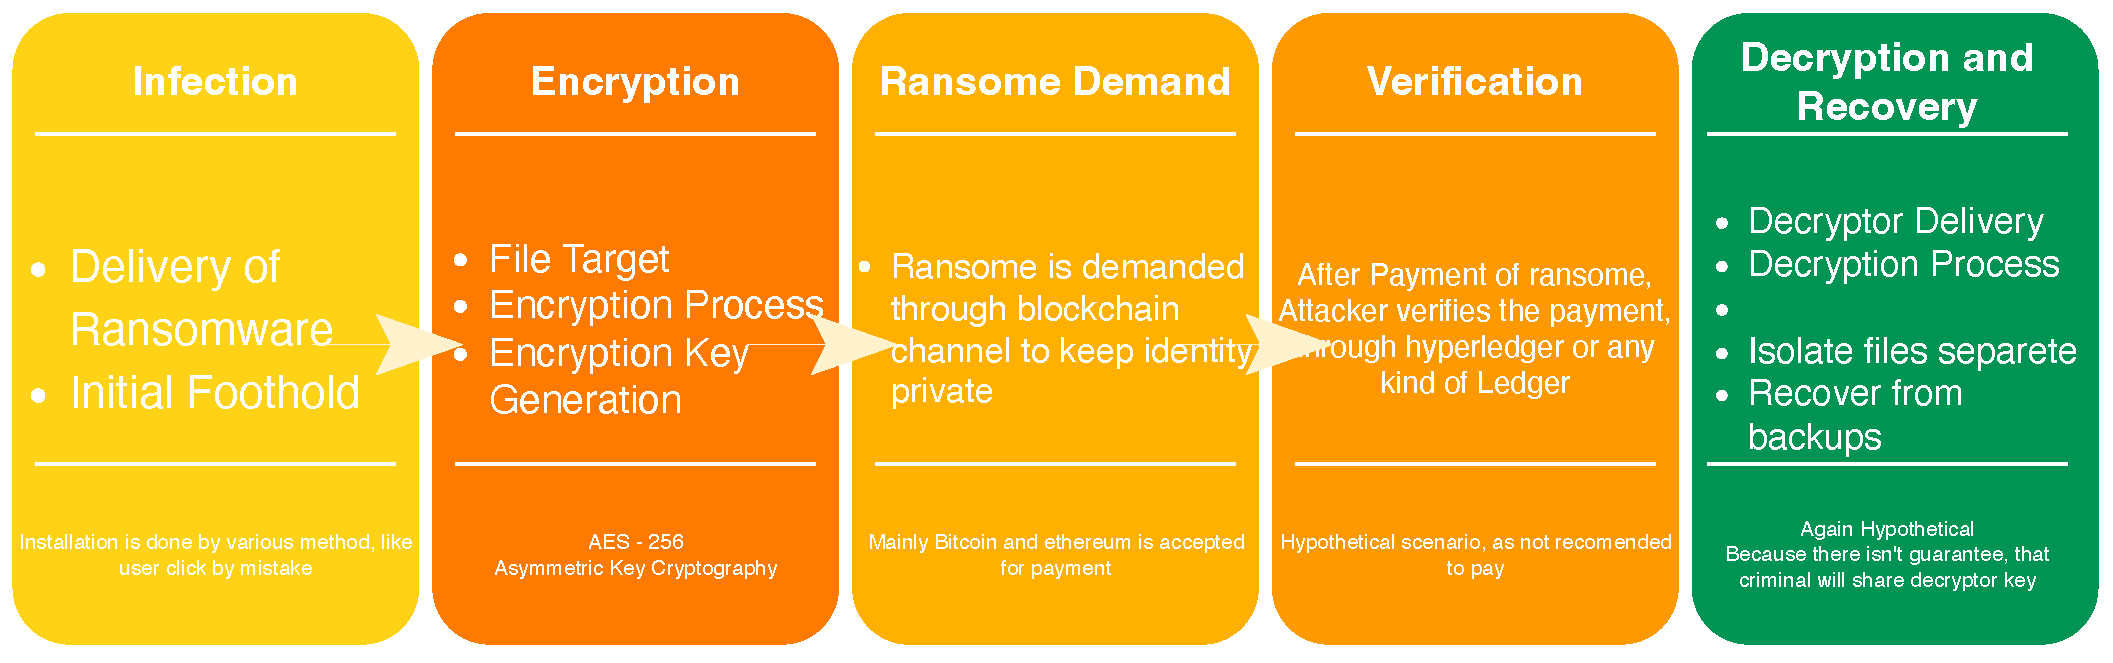
\includegraphics[width=\textwidth]{images/lifecycle.pdf}
            \caption{Depiction of Life Cycle of ransomware}
            \label{fig:Ransomware Lifecycle}
        \end{figure*}
        
        \begin{enumerate}[label=\arabic*.]
        \item Infection:
    
        \begin{enumerate}[label=\alph*.]
            \item Delivery: Ransomware reaches a target system through various methods like phishing emails with malicious attachments, infected websites, RDP (Remote Desktop Protocol) vulnerabilities, or unpatched software.
    
            \item Initial Foothold: Once the ransomware gains access, it exploits vulnerabilities to establish a foothold on the system. This might involve creating new user accounts, disabling security software, or spreading laterally across the network.
            
        \end{enumerate}

        \item Encryption:
    
        \begin{enumerate}[label=\alph*.]
            \item File Targeting: The ransomware identifies and targets critical files and documents on the victim's device or network. This could include financial records, personal data, business documents, or system files.
    
            \item Encryption Process: Using strong encryption algorithms, the ransomware encrypts the targeted files, making them inaccessible to the victim. This process might vary depending on the specific ransomware strain.
    
            \item Encryption Key Generation: During encryption, the ransomware creates a unique decryption key for each victim. This key is essential for regaining access to the encrypted files. However, the attackers keep this key for themselves.
            
        \end{enumerate}
    
        \item Ransom Demand:
    
            Ransom Note: The ransomware displays a ransom note on the victim's screen. This note explains the situation, highlights the urgency, and outlines the attacker's demands. It typically includes instructions on how to pay the ransom, often in cryptocurrency like Bitcoin, due to its anonymity. The note might threaten to permanently delete backups, leak stolen data, or launch further attacks if the ransom isn't paid within a specific time frame.
    
            \item Verification (Hypothetical Scenario):
    
                \begin{enumerate}[label=\alph*.]
                    \item Ransom Payment: If the victim chooses to pay (not recommended), they'd follow the attacker's instructions, which might involve sending cryptocurrency to a specific address.
        
                    \item Verification (Unreliable): In an ideal scenario (which isn't guaranteed with cybercriminals), the attackers might verify the payment received.
                \end{enumerate}
            
            \item Decryption (Hypothetical Scenario):
    
                \begin{enumerate}[label=\alph*.]
                    \item Decryptor Delivery (Unreliable): Again, assuming the attackers keep their word, they might provide a decryptor tool or the unique decryption key to the victim.
    
                    \item Decryption Process: The victim would then use the decryptor or key to decrypt the compromised files and regain access.
                \end{enumerate}
    
        \subsubsection{Safety Precautions and Measures:}
            \item Recovery (Recommended Approach):
                \begin{itemize}
                    \item Isolate Infected Systems: Disconnect affected devices from the network to prevent further spread.
    
                    \item Report the Attack: Inform law enforcement agencies and relevant authorities to assist with investigation and potential recovery efforts.
    
                    \item Restore from Backups: If you have up-to-date backups, restore your critical data from a safe, isolated location.
        
                    \item Remediate Vulnerabilities: Patch software vulnerabilities, update security software, and implement stronger access controls to prevent future attacks.
        
            \end{itemize}
        
        \end{enumerate}

        \subsection{Impact of Ransomware}

        Ransomware attacks have emerged as one of the most significant cybersecurity threats facing individuals, businesses, and organizations worldwide. These malicious incidents not only result in financial losses but also have far-reaching consequences that extend beyond immediate monetary damages. In this section, we explore the multifaceted impact of ransomware attacks on various stakeholders and the broader cybersecurity landscape.

        \begin{enumerate}
            \item \textbf{Financial Losses:} Ransomware attacks inflict substantial financial losses on victims, including ransom payments, remediation costs, and potential revenue disruptions. The direct financial impact of ransomware incidents can be staggering, with ransom demands ranging from hundreds to millions of dollars, depending on the scale and severity of the attack. 

            \item \textbf{Data Breaches and Confidentiality Breaches:} Ransomware attacks often involve the exfiltration of sensitive data from compromised systems, posing a significant risk of data breaches and confidentiality breaches. Cybercriminals may threaten to release or sell stolen data if ransom demands are not met, leading to reputational damage, legal liabilities, and regulatory penalties for affected organizations. The exposure of confidential information can have long-term consequences for individuals and businesses, eroding trust and undermining brand integrity.

            \item \textbf{Operational Distruptions:} The operational disruptions caused by ransomware attacks can have profound implications for business continuity and productivity. Ransomware-induced downtime can paralyze critical systems and services, disrupting day-to-day operations, customer interactions, and supply chain activities. The inability to access essential data and applications hampers decision-making processes and impedes organizational agility, resulting in cascading effects across the entire enterprise.

            \item \textbf{Reputational Damage:} Ransomware attacks can inflict lasting reputational damage on affected organizations, eroding stakeholder trust and confidence. Public disclosure of a ransomware incident can tarnish a company's reputation, leading to loss of customers, partners, and investors. The perception of inadequate cybersecurity measures or mishandling of sensitive data can irreparably harm brand reputation and undermine competitive advantage in the marketplace.

            \item \textbf{Legal and Regulatory Consequences:} Ransomware attacks carry significant legal and regulatory implications for organizations, particularly those operating in regulated industries. Non-compliance with data protection laws and regulations, such as the \ac{GDPR} or the \ac{HIPAA}, can result in severe penalties and sanctions. Organizations may face lawsuits, regulatory investigations, and class-action claims stemming from ransomware-related data breaches, further compounding the fallout from the attack.
        \end{enumerate}

    \clearpage

\newpage
\phantomsection
\section*{Chapter 2}
\addcontentsline{toc}{section}{Chapter 2}
    \section{Literature Review}

    The landscape of ransomware threats continues to evolve rapidly, posing significant challenges to cybersecurity practitioners and researchers alike. As organizations grapple with the escalating frequency and sophistication of ransomware attacks, the need for effective detection and mitigation strategies has become increasingly paramount. In this chapter, we conduct a comprehensive literature review to explore the existing body of research and solutions in the domain of ransomware detection, with a particular focus on the integration of Software-Defined Networking (SDN) technology.

    The motivation for this literature review stems from the urgent need to address the pervasive threat of ransomware attacks and the limitations of traditional networking approaches in combating this menace. Traditional networking architectures, characterized by their reliance on hardware-based infrastructure and distributed control mechanisms, are ill-equipped to cope with the dynamic and evolving nature of modern cyber threats, including ransomware. These legacy systems often lack the agility, scalability, and programmability required to detect and mitigate ransomware attacks effectively.

    Traditional networking approaches suffer from several inherent limitations that hinder their efficacy in ransomware detection and mitigation. These include:

    \begin{enumerate}
        \item \textbf{Heavy and Non-Programmable Infrastructure:} Traditional networking infrastructures consist of complex, hardware-based components, such as routers, switches, and firewalls, that are challenging to manage and configure. The reliance on proprietary hardware limits the flexibility and agility of traditional networks, making them unsuitable for rapidly adapting to changing threat landscapes.

        \item \textbf{Lack of Real-Time Monitoring and Mitigation:} Traditional networking architectures are constrained by their static and reactive nature, making it difficult to detect and respond to ransomware attacks in real-time. The absence of centralized control and orchestration mechanisms impedes the ability to implement dynamic security policies and conduct timely threat analysis, leaving organizations vulnerable to ransomware incidents.
    \end{enumerate}

    In contrast, Software-Defined Networking (SDN) represents a paradigm shift in network architecture, offering a more agile, scalable, and programmable alternative to traditional networking approaches. By decoupling network control and data forwarding functions and centralizing network management through software-defined controllers, SDN enables organizations to overcome the limitations of traditional networking and enhance their cybersecurity posture.
    \clearpage
    \subsection{SDN}

    In traditional networking, data moves across devices like switches and routers through packets, where each device makes forwarding decisions based on its own control logic. This setup integrates the control plane (managing routing protocols) and data plane (forwarding packets) within each device. \cite{nadeau2013sdn}

    Software-Defined Networking (SDN) separates the control plane from the data plane, centralizing control logic in a software-defined controller. This controller communicates with forwarding devices to dynamically configure network behavior. Unlike traditional setups, SDN offers centralized management, dynamic policy enforcement, and greater flexibility in network customization and response to changing conditions.

    \begin{figure*}[ht]
        \centering
        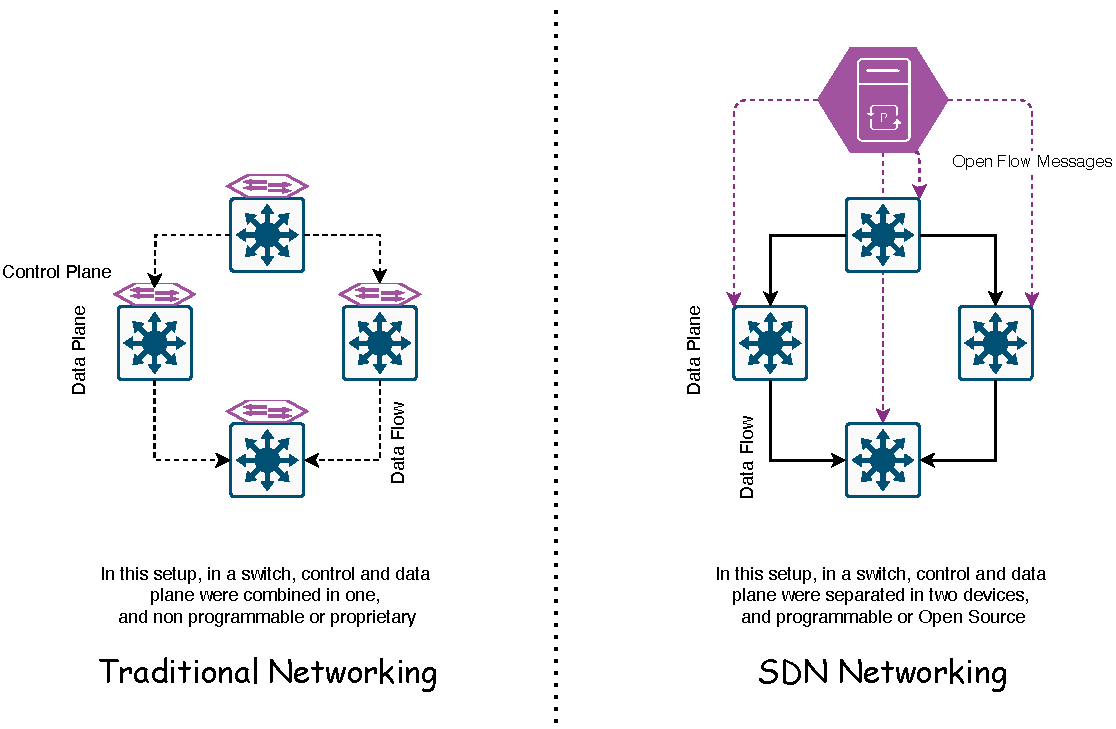
\includegraphics[height = 12 cm]{images/sndvtra.pdf}
        \caption{Differences between Traditional and SDN Networking}
        \label{fig: SDN vs Tranditional Comparision}
    \end{figure*}

    As shown in \autoref{fig: SDN vs Tranditional Comparision}, we can say that, using SDN we can easily manage and manipulate our network flow as per our requirements.

    \subsection{Planes of Network}

    Every single network device typically has to perform three distinct activities, which are mapped correspondingly to three different planes of the network: data, control and management, as depicted in \autoref{fig:Data Flow working Diagram}

    \begin{figure*}
        \centering
        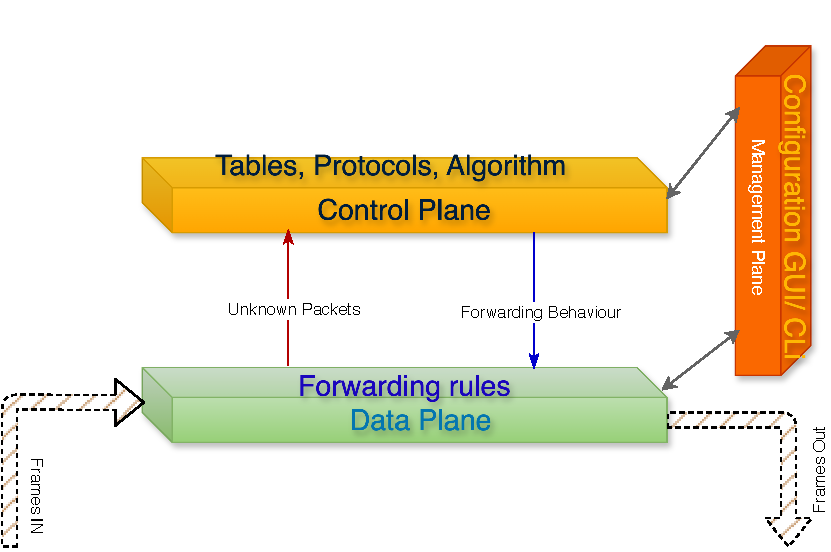
\includegraphics[height= 8cm]{images/Data Flow Diagram.drawio.pdf}
        \caption{Data Flow working Diagram}
        \label{fig:Data Flow working Diagram}
    \end{figure*}

    \subsubsection{Data Plane}

        \begin{itemize}
            \item The data plane is responsible for processing the transit traffic, which decides what to do with packets arriving on an ingress interface.
            \item  It is also termed as forwarding plane, as it mainly refers to a forwarding table to decide proper egress interface.
            \item  From the perspective of packets the data plane usually handle end-station / user-generated packets that are always forwarded by network devices to other end-station devices.

        \end{itemize}

    \subsubsection{Control Plane}

        \begin{itemize}
            \item The control plane is concerned with collecting, processing and managing the network information in order to decide the forwarding behavior.
            
            \item It typically includes various tables and suite of protocols that work on these tables. Hence, control plane handles network device generated/received packets that are used for the creation and operation of the network itself.
                
            \item Typical protocols that run at control plane are routing, interface state management, connectivity management, adjacent device discovery, topology or reachability information exchange and service provisioning.

        \end{itemize}

    \newpage
    \subsubsection{Management Plane}
        \begin{itemize}
            \item The management plane is used to interact, or monitor, with the device, in order to manage the network.
            \item The management plane also runs its own suite of protocols such as \ac{SNMP}, apart from supporting configurations of interfaces, network (IP subnets) and control-plane protocols.
            \item In a traditional network device, the data-plane activities are carried out by dedicated hardware (or ‘high-speed code’), while the control plane operations are handled by the device CPU.

        \end{itemize}

    \section{Basics of Switch}

    \begin{figure*}[ht]
        \centering
        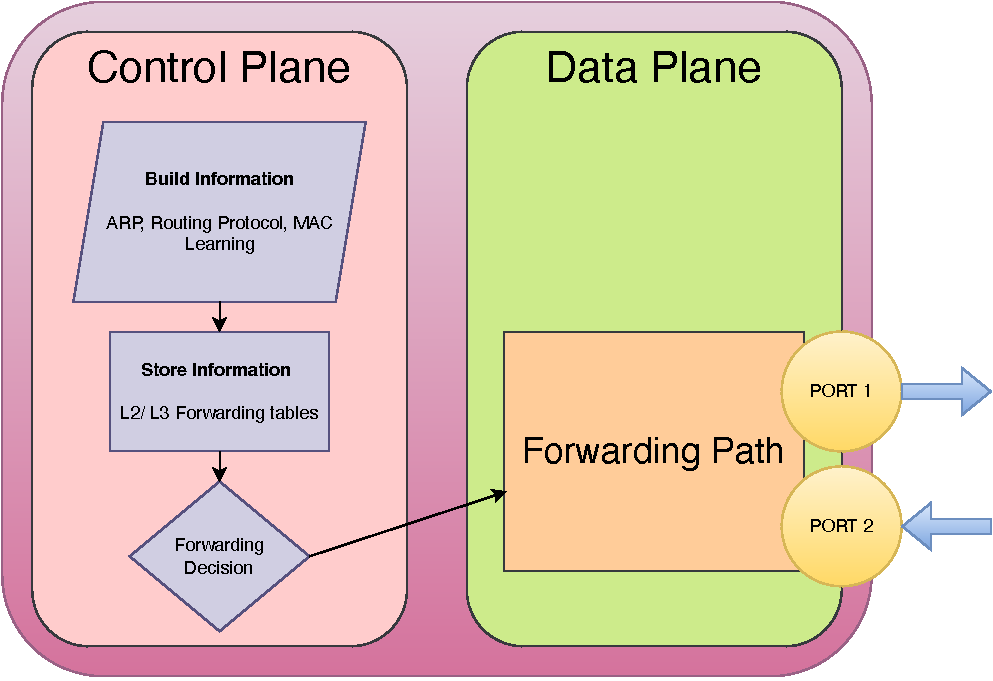
\includegraphics[height = 8 cm]{images/basicSwitch.drawio.pdf}
        \caption{Schematic of Traditional Switch Workings}
        \label{fig:Schematic of Traditional Switch Workings}
    \end{figure*}

    \begin{itemize}
        \item The basic job of a network switch is to make a forwarding decision (control plane) and subsequently forward the data toward a destination (data plane), shown in \autoref{fig:Schematic of Traditional Switch Workings}.
        \item To make forwarding decisions very quickly, the network switch is equipped with very specialized memory resources \ac{TCAM} to hold the forwarding information. The specialized nature of this memory makes it difficult and expensive for each switch to have large quantities of memory available for holding information about a large network.
    \end{itemize}

    \subsection{Traditional Networking}

    \begin{itemize}
        \item  Traditionally, routers/L3 switches have two high-level functionalities:
        \begin{enumerate}
            \item Control-plane functionality (routing protocols, QoS protocols)
            \item Forwarding functionality (high speed forwarding based on rules stored in the forwarding tables)
        \end{enumerate}
        \item Control plane and data plane are coupled!, \autoref{fig:Schematic of Traditional Switch Workings}.

    \end{itemize}


    \subsection{Software Defined Networking}

    \begin{figure*}[ht]
        \centering
        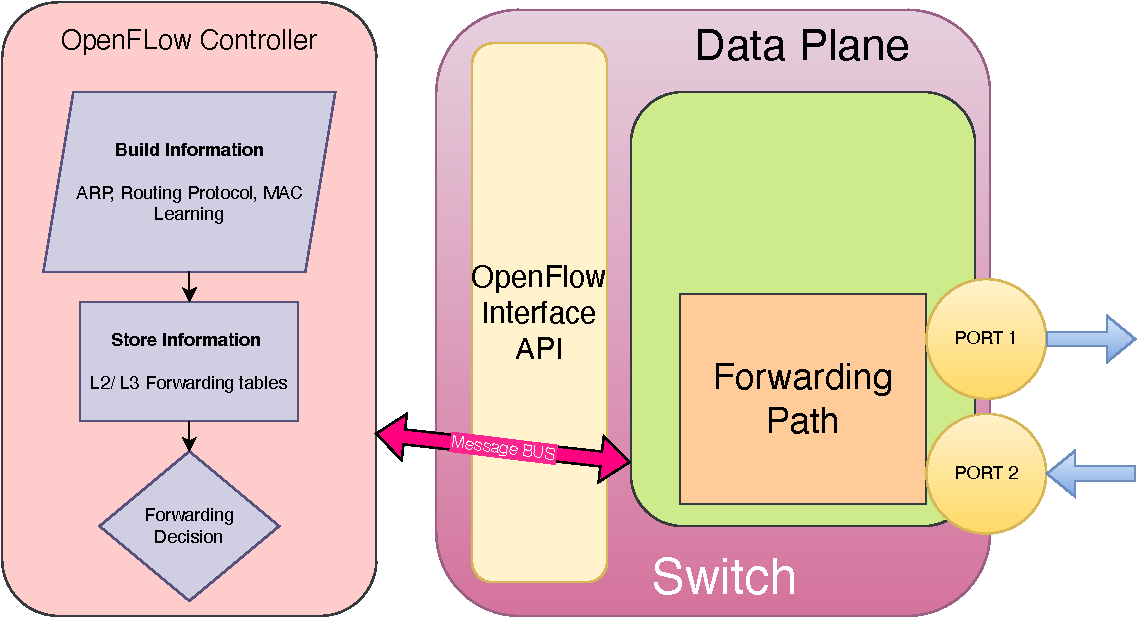
\includegraphics[height=8cm]{images/schematicSDNSw.drawio.pdf}
        \caption{Schematic of SDN Switch}
        \label{fig:Schematic of SDN Switch}
    \end{figure*}

    \begin{itemize}
        \item SDN is about refactoring of the relationship between network devices and the software that controls them. 

        \item Replacing the distributed control-plane with a logically centralized ones, \autoref{fig:Schematic of SDN Switch}.
    \end{itemize}


    \subsection{Overview of SDN vs Traditional Netowrk Setup}

        \begin{table}[ht]
            \centering
            \caption{Comparison of Traditional Network and Software Defined Network}
            \label{tab:network-comparison}
            \begin{tabular}{ccc}
            \toprule
            \textbf{Criteria} & \textbf{Traditional Network} & \textbf{Software Defined Network} \\
            \midrule
                Network Management & Difficult: Apply on each devices & Easy: Centrally Programmable \\
                Global Network View & Difficult & Central View at Controller \\
                Time for update/ Error Handling & Difficult: takes months & Easy: with Software Based \\
                Attack Detection and Mitigation & Difficult & Easier \& Quick \\
                Availablity of Controller & Not Relevent & Important \\
            % Add more rows as needed
            \bottomrule
            \end{tabular}
        \end{table}
\clearpage    
    \newpage
    \section*{Chapter 3}
        \section{Proposed Work}
        In this chapter, we introduce our proposed work. We give a detailed description of our approach and explain the architecture of our model by describing each sub module in detail. We also explain the workflow of our proposed solution through a simple example.

        \subsection{Approach}

            \begin{figure*}[ht]
                \centering
                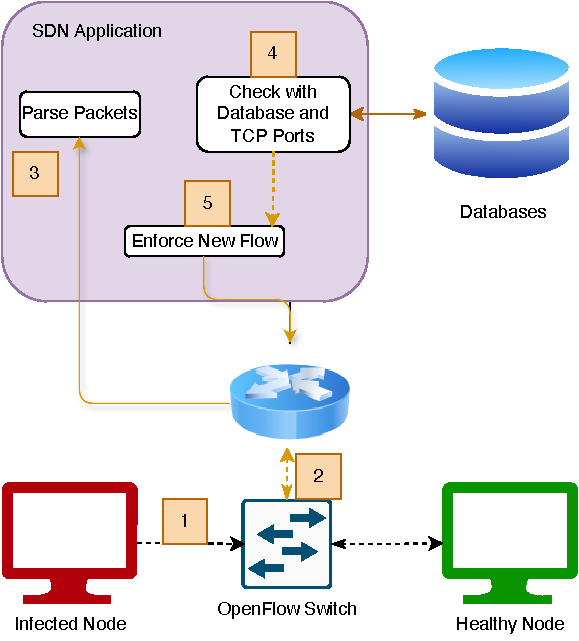
\includegraphics{images/ConceptDesign.drawio.pdf}
                \caption{Conceptual design of the proposed SDN-based mechanism}
                \label{fig:Conceptual design of the proposed SDN-based mechanism}
            \end{figure*}

            Our proposed SDN-based detection and mitigation mechanism relies on inspection of the \ac{DNS} traffic with dynamic black- listing, which particularly observes the network traffic for the presence of malicious domain names or IP addresses used during WannaCry’s communication with the C \& C server. %(as identified in Sections 3 and 4 ). 
            As soon as such an attempt is detected, it is blocked. The list of malicious domain names is commonly specified in a local blacklisting file or by using online databases. One of the main benefits of this method is that it provides simplicity in implementation and effectiveness in detection and mitigation of malware activity. Therefore, this approach was used as a basis for our proposed mechanism.
\\
            The conceptual design of the proposed mechanism is depicted in \autoref{fig:Conceptual design of the proposed SDN-based mechanism}. The main detection and mitigation functionality is carried out by the developed SDN application. This application has been implemented on the SDN controller, which allows inspecting the entire network traffic and issuing instructions to the OpenFlow switch to update its flow table by installing appropriate rules. In \autoref{fig:Conceptual design of the proposed SDN-based mechanism}, numbers 1 to 5 represent different steps of the detection and mitigation process and are explained below:

            \begin{enumerate}
                \item Malicious \ac{TCP} traffic from an infected host arrives to the OpenFlow switch. This traffic includes \ac{SMB} probing and DNS query packets generated by WannaCry.

                \item Assuming that initially there is no flow entry for the given infected host, the switch redirects all TCP traffic to the controller (this is the default action), in order to obtain further instructions on how to handle these packets.

                \item All packets that are received by the controller, are passed to the application. The application performs the fol- lowing functions: parses packets, checks against the blacklist database file, and creates new flow entries in the switch. After receiving the packets, the application parses them in order to find any matches with WannaCry’s inherent network indicators.

                \item The packets are checked against the database file containing the list of IP addresses and simultaneously with any matches to the TCP port numbers used by WannaCry.

                \item If malicious communication is detected, the application creates a new flow entry in the switch instructing it to block the malicious traffic originating from the infected host.
               
            \end{enumerate}


            \begin{table}[ht]
                \centering
                \caption{Entries in the flow table of the OpenFlow switch}
                \label{tab:firewall-rules}
                    \begin{tabular}{ccccccc}
                        \toprule
                \textbf{Rule} & \textbf{Src addr} & \textbf{Src port} & \textbf{Dst addr} & \textbf{Dst port} & \textbf{Protocol} & \textbf{Action} \\
                \midrule
        1 & 10.0.0.1 & 80 & 203.0.113.5 & 443 & TCP & Allow \\
        2 & 10.0.0.2 & 22 & 192.168.1.10 & 1025 & UDP & Deny \\
        3 & 172.27.38.83 & Any & 192.168.1.20 & 53 & Any & Allow \\
        % Add more rows as needed
                \bottomrule
                \end{tabular}
            \end{table}

        For example, the new flow table of the OpenFlow switch may contain the entries shown in \autoref{tab:firewall-rules}. In this case, the IP address 192.168.180.130 was taken from the blacklist database file (Step 3) and the relevant TCP port numbers (445, 139, etc.) are known to be used by the SMB protocol.

    
    \subsection{Static Analysis of WannaCry}

        Static ransomware analysis is a method of examining ransomware code and characteristics without executing the malicious software. By analyzing the ransomware's code structure, file properties, and other attributes, static analysis helps uncover potential indicators of compromise (IOCs), encryption algorithms, and other critical information. This approach assists in understanding the ransomware's functionality and behavior, aiding in the development of detection and mitigation strategies.
    
            \begin{table}[ht]
                \centering
                \caption{WannaCry encryption components: Hashes and file types.}
                \label{tab:WannaCry Exec Components}
                \begin{tabular}{ccccccc}
                    \toprule
                    \textbf{Parameter} & \textbf{Encryption Component} \\
                    \midrule
                    MD5 & c5d40dff30148a6a7a9d091f2a31d7c1 \\
                    SHA1 & e3897618a8189f632459e53f4b3e7459fd7f9917 \\
                    SHA256 & c4f868791586ae4c2d25b0d4bcce85b8bef5f5b673d471de2e743156e9e8dfaf \\
                    File Type & PE32+ executable (GUI) x86-64, for MS Windows \\
                    % Add more rows as needed
                    \bottomrule
                \end{tabular}
            \end{table}

            \begin{table}[htbp]
                \centering
                \caption{WannaCry worm components: Hashes and file types.}
                \label{tab:WannaCry Worm Components}
                \begin{tabular}{ccccccc}
                    \toprule
                    \textbf{Parameter} & \textbf{Worm Component} \\
                    \midrule
                    MD5 & e8a30656287fe831c9782204ed10cd68 \\
                    SHA1 & e3897618a8189f632459e53f4b3e7459fd7f9917 \\
                    SHA256 & 4625f4c125f3ce2cd4d2c8365d2996bfed67a0f545e08c215307edf944b3af88 \\
                    File Type & PE32+ executable (GUI) x86-64, for MS Windows \\
                    % Add more rows as needed
                    \bottomrule
                \end{tabular}
            \end{table}

        We analyzed two WannaCry executables: the worm component and the
        encryption component. Their corresponding hashes and basic characteristics are shown in \autoref{tab:WannaCry Exec Components} and \autoref{tab:WannaCry Worm Components}. Below we present our main findings from the static 175 analysis.
        Analysis with the Pestudio tool has revealed that the worm and the en-cryption components contain dynamic-link libraries (DLLs), as shown in \autoref{tab:DLL-Link File} and \autoref{tab:DLL-Link1 File}. During its execution, the worm invokes the iphlpapi.dll in order to retrieve network confguration settings for the infected host. The kernel32.dll 180 and msvcrt.dll are two most invoked libraries by the encrypter. It was found that WannaCry uses Microsoft's crypto, file management, and C runtime file \ac{API}. The Crypto API library is used to generate and manage random symmetric and asymmetric cryptographic keys.


        \begin{table}[ht]
            \centering
            \caption{Dynamic Link Libraries (DLLs) invoked by WannaCry's encryption component}
            \label{tab:DLL-Link File}
            \begin{tabular}{ccc}
                \toprule
                \textbf{Library} & \textbf{Imports} & \textbf{Descriptions} \\
                \midrule
                USERS32.dll & 2& Multi-UserWindows USER API Client\\
                KERNEL32.dll & 10& Windows NT BASE API Client\\
                ADVAPI32.dll & 1& Advanced Windows 32 Base API\\
                WS2\_32.dll & 1& Winsock DLL Loading\\
                % Add more rows as needed
                \bottomrule
            \end{tabular}
        \end{table}

        \begin{table}[ht]
            \centering
            \caption{Dynamic Link Libraries (DLLs) invoked by WannaCry's worm component}
            \label{tab:DLL-Link1 File}
            \begin{tabular}{ccc}
                \toprule
                \textbf{Library} & \textbf{Imports} & \textbf{Descriptions} \\
                \midrule
                USERS32.dll & 2& Multi-UserWindows USER API Client\\
                KERNEL32.dll & 10& Windows NT BASE API Client\\
                ADVAPI32.dll & 1& Advanced Windows 32 Base API\\
                WS2\_32.dll & 1& Winsock DLL Loading\\
                msvcp60.dll & 2 &  Windows NT C++ Runtime Library \\
                msvcrt.dll & 28 & Windows NT CRT \\
                % Add more rows as needed
                \bottomrule
            \end{tabular}
        \end{table}


    \subsection{Dynamic Analysis of Ransomware}

    % Our dynamic analysis has revealed that, when started, the worm component invokes the \textit{InernetOpenUrl} function and attempts to establish a connection with the following domain

    Dynamic analysis of WannaCry was conducted in a virtual test environment. A custom network was created to monitor DNS queries made by the ransomware across internal and external networks via port 445. The REMnux machine served as a DNS and HTTP server, intercepting network communications using Wireshark. The analysis showed that the ransomware attempted to connect to a specific domain upon startup using the \textit{InernetOpenUrl} function: \url{ieonline.microsoft.com}, as shown in \autoref{fig:fakedns-capture} we have verified that there is no such domain is mentioned in official Microsoft Support \url{https://learn.microsoft.com/en-us/windows/privacy/manage-windows-1903-endpoints}.

    \begin{figure}[hbtt]
        \centering
        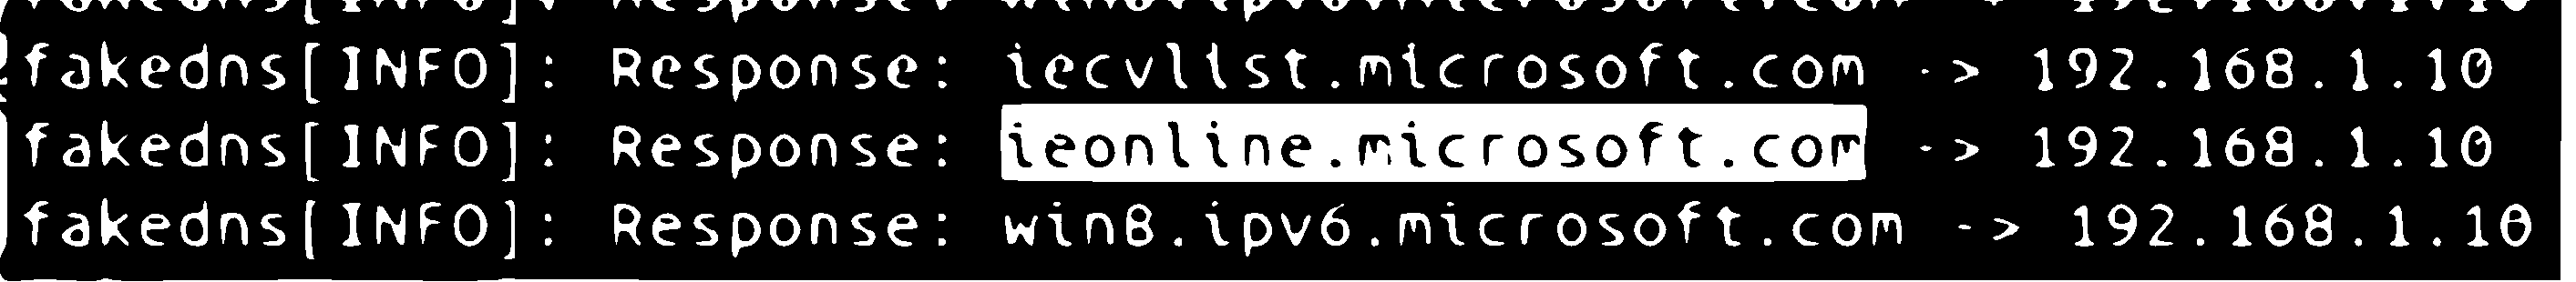
\includegraphics[width= \textwidth]{images/urlfakedns.pdf}
        \caption{FakeDNS Captured Domain Name}
        \label{fig:fakedns-capture}
    \end{figure}

    We have also found that, in the DNS record, our ransomware ping maximum numbers of times url is \url{dns.msftncsi.com}, which is unusual for request, as per Pi-Hole Website \cite{pi-hole}, it is seen that many request are made.

    Our analysis has also shown that WannaCry attempts to establish persistence on the infected device by: 

    \begin{itemize}
 
        \item Creating an entry in the Windows registry, so that it is invoked every time the infected computer reboots.
        
        \item Adding itself to the AutoRun feature of Windows. 

        \item  Utilizing the icacls command to enable full access to all files on the infected device.

        \item  Deleting the backup copies and preventing the device rebooting in the safe mode.

        \item Attempting to eliminate SQL and MS Exchange database processes by executing certain shell commands.
        
    \end{itemize}

    \subsubsection{Challenges of dynamic malware analysis}

    \begin{itemize}
        
        \item Dynamic malware analysis is more time-consuming and resource-intensive than static analysis. It can also pose a threat if the virtual environment is not completely isolated from other systems.

        \item Additionally, while executing the malware helps teams understand more about a sample, it can also alert malware authors when their samples run.

        \item Sophisticated malware can also sometimes detect when it is executed inside an isolated virtual environment instead of a natural environment. It does this by observing registry keys, processes or even whether the mouse and keyboard are actively in use. Some malware that can identify the difference might also employ techniques to prevent accurate analysis. It is challenging to create a realistic sandbox that can fool sophisticated malware, but it certainly isn't safe to execute a malware sample on a live system.
    \end{itemize}
    
    \subsection{Approach To Detect}

        Since we using SDN approach to blocking ransomware to spread by using counter measures by blocking host in network on basis of Capturing malicious operation like SMB exploitation and pinging unwanted/ unverified Domain Name and IP Address.

        But this working model already done with firewall, so we adapted new approach i.e., \ac{DPI} \cite{enwiki:1223318045}, based on the concept, this process will capture the packet in real time in control plane of the network, which is actually a pox controller, then it will match the pattern of signature with pre-existing samples, or if sample is not available then check for any piece of code in packets which seems to be malicious in nature, like containing any kinds of crypto-currency addresses, or contains any functions which is calling kernel level objects, as we learnt in static analysis of malware.

        After proper identification of packets, the detection system will notify the POX controller to block the particular host, in a network, because it might be possible, as we assumed the scenario that some legitimate users in network, can also share ransomware files as shown in \autoref{fig:legitimate Scenario}.

        The applied algorithm and approach are show in \autoref{Checking and Analysing Packets}

        \begin{figure}[ht]
            \centering
            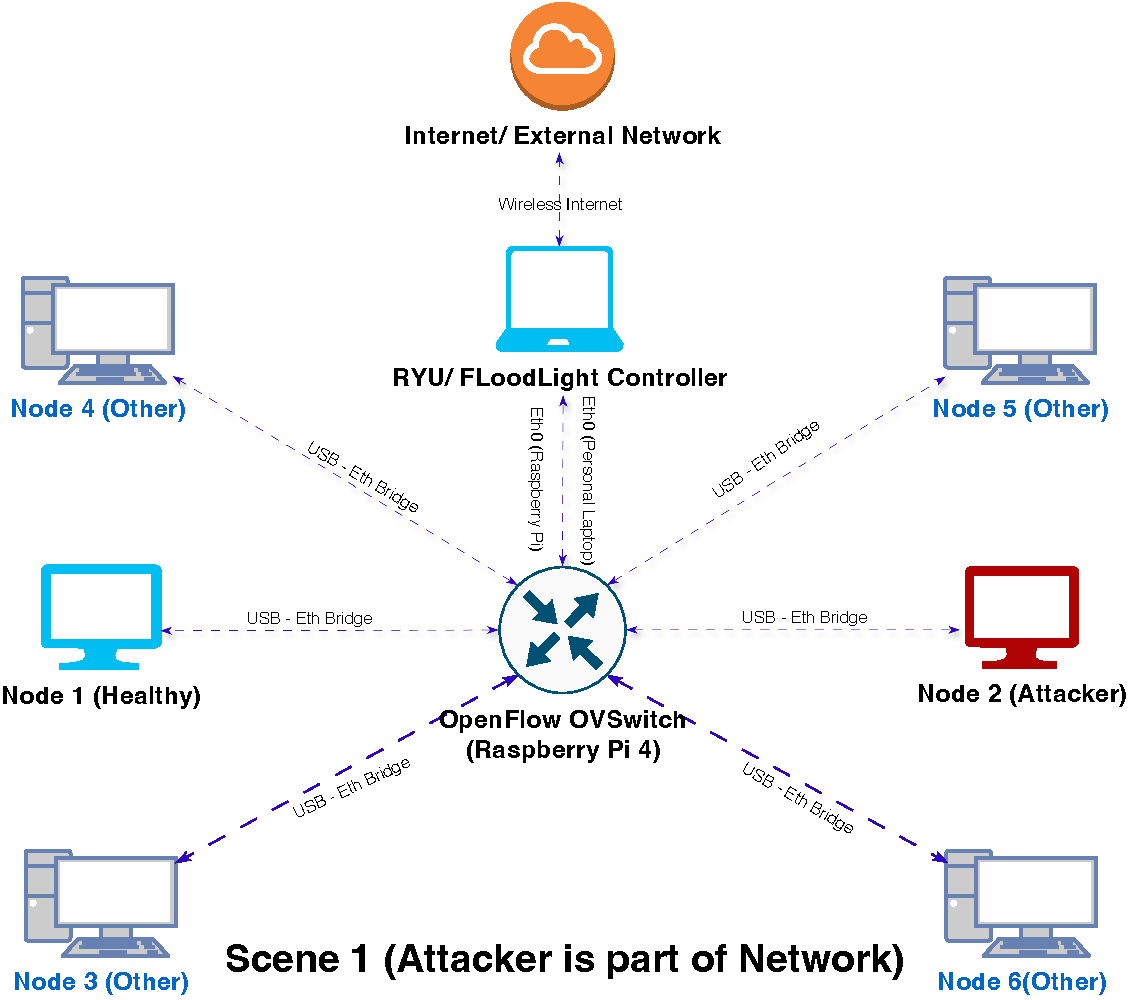
\includegraphics[height = 8cm]{images/Scene1.pdf}
            \caption{Legitimate node become attacker}
            \label{fig:legitimate Scenario}
        \end{figure}

        \subsection{Overview of Deep Packets Inspection}

        \textit{Deep packet inspection (DPI)}, alternatively referred to as information extraction or complete packet inspection, serves as a comprehensive form of network packet filtering. It scrutinizes both the data and header sections of transmitted packets at inspection points, identifying and filtering out any content that violates protocol standards or poses security risks, such as spam, viruses, and intrusions.
        
        Furthermore, DPI plays a pivotal role in directing packets to their intended destinations. In essence, it possesses the capability to identify, categorize, block, or reroute packets containing specific code or data payloads that might evade detection or redirection by conventional packet filtering methods. Unlike traditional packet filtering, DPI delves deeper into packet contents beyond mere header examination.

        The most common inspection used consists in comparing the packet content against certain attributes and checking for hits in any of the accessible layers. Depending on the application in which DPI is used the inspection process could be customized in terms of what needs to be matched, such as traffic from a certain IP address etc. DPI includes port-based analysis that enables the identification of the port number by inspecting the \textbf{TCP} or \textbf{UDP} headers and thus determining which protocol was used to generate the packet. Statistical analysis can also be employed as a DPI method, but it is not payload specific and rather uses several approaches to classify traffic based on port numbers or timestamps. We argue, however, that both port-based and statistical analysis methods are not exactly DPI but could be classified as what is known as \ac{SPI} \textcite{mochalski2009} because the payload is not involved at any stage of the inspection process. 

        There exist multiple DPI methods, the variation is determined based on how the payload is matched to keywords. Understanding the logic behind DPI is an important step to find out which method should be avoided and which can be improved. Some of the methods can be performed as either string matching or regular expression matching \textcite{Xu2016ASO}. We are mainly interested in two methods and the ones that are most commonly used among all \textcite{Xu2016ASO}, they are as follows:

        \subsubsection{Comparison of Deep Packet inspection vs Conventional Inspection}

        \begin{table}[ht]
    \centering
    \caption{Comparison of Deep Packet Inspection vs Conventional Packet Filtering}
    \label{table:comparison}
    \begin{tabular}{p{0.45\linewidth} p{0.45\linewidth}}
        \toprule
        \textbf{Conventional Packet Filtering} & \textbf{Deep Packet Inspection (DPI)} \\
        \midrule
        Reads only the header information of each packet. & Analyzes both the header and data sections of packets. \\
        Limited in sophistication due to technology constraints. & Enabled by advancements in technology, allowing for more thorough analysis. \\
        Similar to reading the title of a book without evaluating the content inside. & Comparable to picking up a book, cracking it open, and reading it from cover to cover. \\
        Less effective in detecting complex threats and security risks. & More comprehensive, capable of identifying and blocking sophisticated threats, such as malware and intrusions. \\
        Often used in basic firewall configurations. & Deployed in modern security systems for enhanced threat detection and prevention. \\
        \bottomrule
    \end{tabular}
\end{table}


        \subsubsection{Limitation of our approach}

            While our approach offers significant advantages in terms of security enhancement, it's important to acknowledge several limitations that may arise. These include:

            \begin{enumerate}
                \item Deep packet inspection stands as a formidable defense against various cyber threats, including denial of service attacks, buffer overflow attacks, and certain types of malware. However, it also holds the potential for crafting similar attacks.

                \item While offering enhanced security, deep packet inspection adds complexity to existing firewall and security software setups. Regular updates and policy reviews are essential to maintain its efficacy.

                \item The rigorous scrutiny involved in deep packet inspection can introduce network latency by necessitating significant resource allocation. Storing packets temporarily for analysis may further contribute to delays in transmission and reception. Leveraging pre-existing samples from past network communications could expedite packet processing decisions.
                
            \end{enumerate}

    \subsection{Results}

    In this work, we present our ransomware analysis results and our developed SDN-based security framework. For the proof of concept, the infamous WannaCry ransomware is used. However, the developed framework is also applicable in other ransomware families. In particular, we examine the behaviour of WannaCry during its execution in an isolated virtual lab environment. Based on the obtained results, we design an SDN detection and mitigation framework and develop a solution based on OpenFlow \cite{10.1145/1355734.1355746, KazuyaSUZUKI2014}, which is currently the most widely adopted SDN standard. The developed solution detects suspicious activities through network traffic monitoring and blocks infected hosts by adding flow table entries into Open- Flow switches in a real-time manner. The logic of the proposed framework has been implemented in the POX controller. For detection purposes, our implementation utilizes the WannaCry’s features and its generated traffic. Finally, our experimental results with multiple samples of WannaCry show that the developed mechanism is able to promptly detect, in all cases, the infected machines and prevent WannaCry from spreading.

    The developed system is able to detect malicious activities using real time traffic analysis. Ceron et al. \cite{7543792} design and develop an SDN based malware analysis system which is capable to dynamically modify the network environment based on malicious activities. It has been demonstrated that the developed solution could trigger more malware events than traditional solutions.

    This solution utilizes an application written for the POX controller, which connects to a blacklist database and performs dynamic checks on IP addresses. The main drawback of these approaches is the requirement to pre-define the ransomware proxy servers used in the blacklisting.

    The feasibility of the proposed approaches has been confirmed by implementing and obtaining experimental results based on OpenvSwitch and POX. In particular, simulation results show a detection rate of 97–98\% with only 4–5\% false positives when relying on blacklisted domains.
            
\clearpage    
    \newpage
    \section*{Chapter 4}
        \section{Detailed Info}

            In this section, we provide a comprehensive overview of our research endeavors, focusing on the development and analysis of ransomware. Our work involved the creation of a sophisticated ransomware framework, followed by thorough static and dynamic analysis conducted within a secure sandbox environment. Through meticulous examination and experimentation, we gained valuable insights into the behavior and impact of ransomware, shedding light on its modus operandi and potential mitigation strategies. The following subsections delve deeper into each aspect of our research, detailing the methodologies employed and the key findings obtained.
            
            
        \subsection{Experimental Setup}

        \begin{figure}[htt]
            \centering
            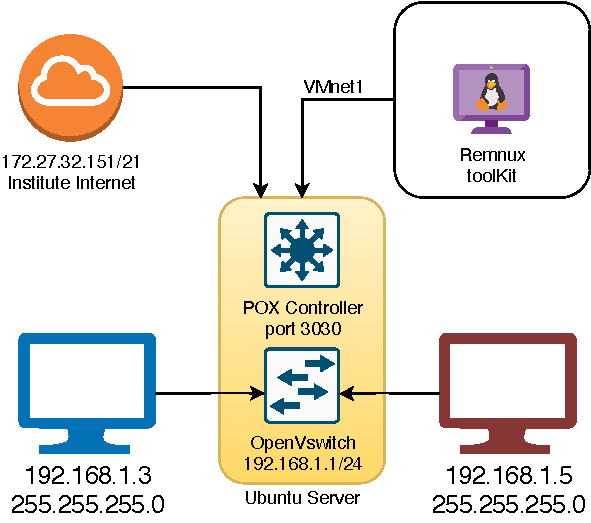
\includegraphics{images/NetworkSetip.drawio.pdf}
            \caption{Network Setup and Connection for Experiment}
            \label{fig:Network Setup and Connection for Experiment}
        \end{figure}

        The network configuration entails the utilization of two physical Windows nodes in conjunction with a singular Ubuntu server, tasked with fulfilling the roles of both the \textbf{OpenVswitch} and \textbf{POX Controller}. This amalgamation is necessitated by constraints in hardware availability or the unavailability of multiple computing units.

        For the Ubuntu Server, a hardware configuration comprising an Intel Core i5 - 4\textsuperscript{th} Generation processor, accompanied by 12GB of RAM, has been employed. Node 1 is equipped with an Intel Pentium 4 processor and 4GB of RAM, while Node 2 features an Intel Core i5 - 8\textsuperscript{th} Generation processor with 8GB of RAM.


        \subsection{Creation of Ransomware}

        

        \subsection{Creation of Trojan Horse}

        In the process of creating the Trojan file for our ransomware, we employed a technique known as \textit{steganography}. This method involves concealing binary data within an image file, allowing the malicious payload to remain undetected by users and security systems alike. By embedding the ransomware binary bits within the pixels of an innocuous-looking image, we aimed to facilitate the covert distribution of the Trojan file. This approach not only enhances the stealthiness of the ransomware, but also increases the likelihood of it being inadvertently triggered by unsuspecting users, thereby maximizing its effectiveness in carrying out its malicious objectives.

        \subsection{Setting up Switch and Controller}

        We follows the following methods, to setup software Based Switch and Controller.

        \subsection{Checking and Analysing Packets}
            \label{Checking and Analysing Packets}




            
        \subsection{Applying Algorithm to Detect and Block}
            \label{Applying Algorithm to Detect and Block}
        
\clearpage
    \newpage
    \section*{Chapter 5}
        \section{Conclusion and Future Scope}

            We'll Write in final Submission

\clearpage
\newpage
\phantomsection
    \printbibliography
    \addcontentsline{toc}{section}{References}

    
% \section*{Team Details}
% \subsection*{Hemant Kumar}
% I am currently pursuing my B.Tech in Computer Science and Engineering from the Indian Institute of Information Technology, Design and Manufacturing (IIITDM) Jabalpur, India, and am in my final year of study. As part of my academic curriculum, I am working on this project/report, which is a requirement for the partial fulfillment of my degree. My research interests include areas such as software engineering, SDN, Social Network Analysis and cybersecurity. %I actively participate in academic and research activities within my institute, and I am eager to contribute to the advancement of knowledge in my field.

% \subsection*{Chaitanya Mandi}
% I am currently pursuing my B.Tech in Computer Science and Engineering from the Indian Institute of Information Technology, Design and Manufacturing (IIITDM) Jabalpur, India, and am in my final year of study. As part of my academic curriculum, I am working on this project/report, which is a requirement for the partial fulfillment of my degree. My research interests include areas such as software engineering, SDN, Social Network Analysis and cybersecurity.
\end{document}